\chapter{Conclusion}

While load balancing and local timestepping certainly display great promise for the acceleration of hurricane storm surge, their implementation in a storm surge code is left as future work. In this chapter we conclude with an analysis of the impact of this work on hurricane storm surge, examine local timestepping through a Tao of parallelism analysis~\cite{Pingali2011}, and conclude with thoughts on storm surge simulations in post-Moore's era computing.

\section{Implications for hurricane storm surge}
In order to make the DG method viable for hurricane storm surge, we require a reduction in required compute resources to still complete a storm surge simulation within a two hour time window. While the proposed local timestepping method represents a significant building block towards using adaptive local timestepping for the simulation of hurricane storm surge, the method must be extended in several important ways. Firstly, the method must be extended to higher-order timestepping schemes. Both partitioned Runge-Kutta methods~\cite{Constantinescu2007} and the extrapolation based methods in~\cite{Hoang2019} offer potential means of achieving this. The high order timestepping schemes extend straightforwardly to the  generalized event trace setting. However, mapping these methods onto a parallel discrete event engine requires more work. Firstly, the extension to multiple dimensions is non-trivial. In the proof of correctness, we showed that a submesh would only send a single message to its neighbor per timestep. This was a result of assuming that the minimum diameter of the submeshes was least two cells. In a multi-dimensional setting, it is possible that a submesh updates, sends unforced push fluxes to a neighbor, and then receives a neighboring push flux that forces the other neighbors to update even though they have already received a push flux. This requires additional control flow as well as incorporation of these states into the proof of correctness.
The second issue arises due to the presence of multiple Runge-Kutta stages per timestep as well as multiple halo-exchanges within a given Runge-Kutta stage. For a given timestepping method these exchanges are statically determined. These message exchanges can be thought of a static task-graph (determined at compile time) embedded inside a dynamic task-graph (determined based on the state of the cell). When executing the tasks inside a static task-subgraph, we know precisely what messages need to be processed before progress can be made. During these portions of the algorithm, any speculation will be rolled back, and insofar we should always wait on these messages. Better abstractions for embedding subgraphs inside a speculative execution context would simplify algorithm development.

\begin{figure}
  \centering
  \subfloat[Element sizes]{\includegraphics{{work_estimate_storm36/h_distribution}.pdf}}\hfill
  \subfloat[Wet fraction]{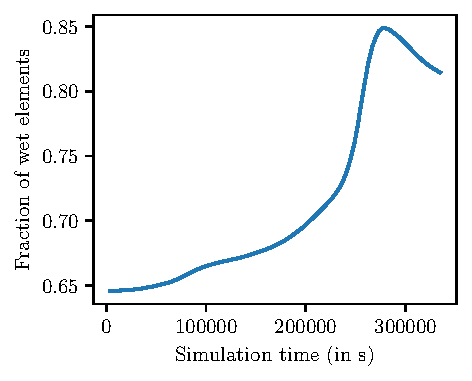
\includegraphics{{work_estimate_storm36/wet_fraction}.pdf}}
  \caption{Storm36 metadata}
  \label{fig:param}
\end{figure}

\begin{figure}
  \centering
  \subfloat[$t=2\,\mathrm{hr}$\label{fig:dt-dist:pre}]{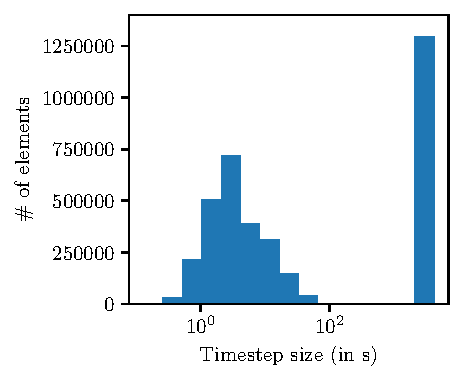
\includegraphics{{work_estimate_storm36/t_distribution7200}.pdf}}\hfill
  \subfloat[$t=77\,\mathrm{hr}$\label{fig:dt-dist:post}]{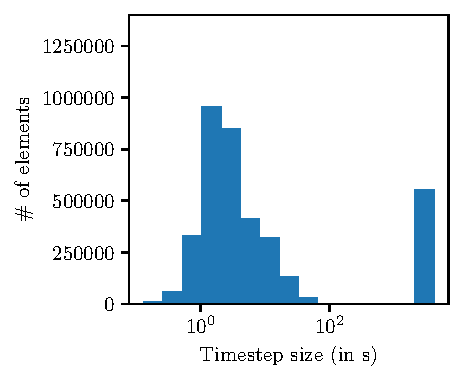
\includegraphics{{work_estimate_storm36/t_distribution277200}.pdf}}
  \caption{Timestep distribution during Storm36}
  \label{fig:dt-dist}
\end{figure}

\begin{figure}
  \centering
  \includegraphics{{work_estimate_storm36/work_contour}.pdf}
  \caption{Work distribution during Storm36}
  \label{fig:w-contour}
\end{figure}

Although high order adaptive local timestepping is a topic of current research, we can use the performance model developed in Chapter~\ref{ch:lts} to approximate the speed-up for a hurricane storm surge simulation. Here we use an ADCIRC solution to the Storm36 problem considered in Chapter~\ref{ch:lb} to compute the wavespeed $|\Lambda|$ at each element. The simulation is run for 3.75 days and the output is recorded hourly. Figure~\ref{fig:param} shows both the wet fraction as well as the distribution of length scales $h$, the inscribed radius of a given element. The mesh contains 3.6 million elements with $h$ ranging from $5.5\,\mathrm{m}$ to $8.5\,\mathrm{km}$. We use the output to compute $|\Lambda|$ and determine the theoretical speed-up $S^{th}$. Based on the minimum inscribed radius and assuming a CFL number of 1/3, we determine the largest stable timestep to be $0.13 \,\mathrm{s}$ and bin the remaining timesteps relative to this $\Delta t_{\min}$. 
 Figure~\ref{fig:dt-dist} shows the distribution of timesteps for both before the storm makes landfall and at peak inundation. In Figure~\ref{fig:dt-dist:pre}, only $0.1\%$ of elements are required to take a timestep of $\Delta t_{\min}$, and the median timestep size is $4.16\,\mathrm{s}$ ($32 \Delta t_{\min}$). As the storm makes landfall in Figure~\ref{fig:dt-dist:post}, the number of elements in the finest timestepping group remains low at $0.3\%$. However signficant inundation has occured. Dry cells are binned into a timestep of 1 hour. The number of cells in this timestepping group has decreased from $35.4\%$ to $15.1\%$ and the median timestep size has also decreased to $2.08\,\mathrm{s}$ ($16 \Delta t_{\min}$). To highlight the small number of cells at the finest timestepping level, we present the work $w_j$ at every thousandth element as a function of simulation time in Figure~\ref{fig:w-contour}. We have intentionally left the colorbar scale linear to highlight that a very small percentage of the elements requires stepping at the finest level. With this information, we can compute the theoretical speed-up $S^{th}$ to be 15.1. Importantly, this number will be smaller in practice since the actual timestep size will also depend on other elements in the given submesh. The discrepancy in expected speed-up computed from \cite{Dawson2013} to the number presented here is due to the fact that in \cite{Dawson2013} the number of timestepping groups was limited to 4 and they used a different mesh. The stability results associated with our adaptive timestepping scheme make this algorithm a good candidate for hurricane storm surge. With proper limiting of bad speculation, we can run the simulation in an almost task-graph manner. Causality violations are relatively rare, yet continuously occurring, making semi-static re-assignment of timestepping groups non-viable. One important question that remains is what is the available parallelism in the simulation? Does our speculative approach bypass the limitations of the adaptive timestepping method, which requires a synchronization after each $\Delta t_{\min}$? This is certainly a lower bound to the amount of available parallelism. On the upper end of parallelism, we are constrained by the parallelism available in the event trace, which is only known a posteriori. These performance analyses are the subject of future work.

%%\subsection{Compute work estimate for any hurricane}
%%Try to come up with impact on time to solution

\section{Tao analysis of adaptive timestepping}
The tao of parallelism categorizes algorithms based on salient features to guide parallel implementations~\cite{Pingali2011}. Programs are thought of as a graph of abstract data types (ADT) and algorithms. In the case of DG finite element methods, the abstract data types correspond to the submeshes, and the edges of the graph are used to reason about dependencies, i.e. which flux buffers need to have been processed before proceeding. The algorithm corresponds to the timestepping scheme, which exchanges flux buffers and updates elements.
The tao analysis then examines three main features shown in Figure~\ref{fig:tao-analysis}.

\begin{figure}
\centering
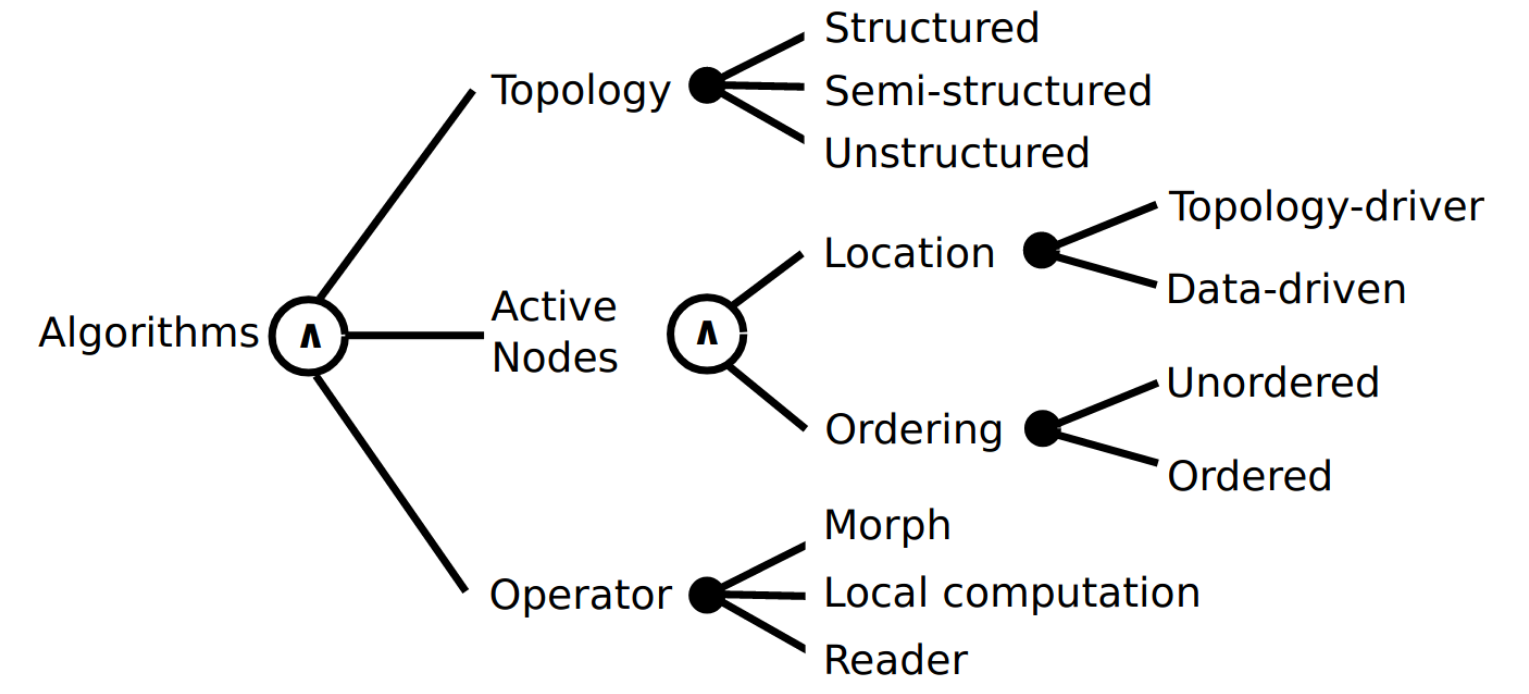
\includegraphics[height=0.25 \textheight]{work_estimate_storm36/tao.png}
\caption{Tao classification of parallel algorithms\cite{Pingali2011}}
\label{fig:tao-analysis}
\end{figure}

\begin{itemize}
\item {\bf T}opology: The topology refers to the ADT graph, for example, if a task is embarrassingly parallel, this might be represented as a graph with an empty edge set. Graphs are classified by the amount of information required to describe them, ranging from structured to semi-structured to unstructured. For our work, we consider the submesh graph generated by the partitioning of a dual graph of a planar mesh. The most important invariant of the graph is that it remains static throughout the simulation. Since we are able to utilize this information to guarantee once an event can be safely processed, we refer to the graph as semi-structured.
\item {\bf A}ctive nodes: At any given point in the simulation, active nodes are nodes which may perform  compute. In the case of the task-based synchronous timestepping, a submesh may only update once it has received the updated boundary state from each of the submesh's neighbors, i.e. once all of its dependencies have been satisfied. The topic of active nodes is split into two further subcategories, {\em location} and {\em ordering}. Location emphasizes whether the active nodes are purely determined by the graph (referred to as topology-driven) or if the state also influences whether or not the algorithm is able to advance (referred to as data-driven). For both synchronous and adaptive local timestepping algorithms, the methods are data-driven. Based on whether or not a submesh has processed a message determines whether or not it can advance to the next timestep. The second subcategory is {\em ordering}. Timestepping methods are inherently ordered. It is nonsensical to have a submesh update in a non-sequential order.
\item {\bf O}perator: Operators are applied to the ADTs. If the operator changes the topology of the graph it is classified as {\em morph}. A {\em local computation} updates the state of the ADT, and a {\em reader} changes neither the state nor the topology. All of our timestepping methods are local computations. Updating the state does not introduce new vertices into the ADT graph.
\end{itemize}
All three timestepping schemes for hurricane storms surge---asynchronous timestepping with a fixed timestep, asynchronous local timestepping, and synchronous timestepping with an adaptive timestep---rely one the same underlying ADT, with an irregular static topology, consist of operators that perform local computation, and have data-driven ordered active nodes. To distinguish between the types of parallelism between each of the timestepping scheme, we rely on the further classification of ordered algorithms by Hassaan~\cite{Hassaan2015, Hassaan2016}. Hassaan introduces the notion of a {\em Kinetic Dependence Graph} (KDG) to classify ordered algorithms. The KDG is defined by a triple $(G,P,U)$, where:
\begin{itemize}
\item $G$ is the task graph,
\item $P$ is a {\em safe source test},
\item $U$ is an update rule.
\end{itemize}
The task graph looks similar to the graph associated with the ADTs, except that in this case directed edges correspond to the next pending flux buffer exchange. The update rule corresponds to the method for updating the ADT, i.e. stepping the mesh forward in time. The key distinction between the three timestepping methods comes from the safe source test. Given an active node of the graph, i.e. a submesh that can be updated, this function examines the graph, and determines whether or not that submesh can locally update. If the safe source test is trivial, any active node can update in parallel and the method is called {\em source stable}.

Coming back to the timestepping schemes, the asynchronous fixed timestepping algorithm is an example of a source stable KDG. Once all messages have been processed at a timestamp, we can safely---here in reference to the algorithm, not the numerical stability---advance to the next timestep. This importantly is contrasted with the other two methods in which case a non-local condition (the CFL condition) needs to be satisfied in order to ensure that the submesh can be safely updated, i.e. the currently proposed timestep will not need to be shortened. Note that the need to check the safety of an update arises due to the fact the shallow water equations are non-linear. Mathematically, the safe-source test requires examining the state of the full domain of dependence. For linear systems of equations, this problem is statically determined, and so timesteps can be proposed (even local timesteps) such that the source test can be guaranteed to be satisfied by construction.

For the synchronous adaptive timestep, the safe source test simply checks all cells, ensuring that the domain of dependence at the proposed timestep is inside the region checked by the safe source test. On the other hand, for the speculative adaptive local timestepping algorithm, we assume that generally the source test will evaluate to true and then rollback in the case that that assumption was incorrect. The performance optimizations outlined in Section~\ref{sec:performance-optimization} then provide two important limitations to bad speculation. The {\em Reducing unnecessary speculation} fix can be thought of as tighter policing of which nodes are active. This fix acknowledges outstanding push fluxes from neighbors as dependencies, and so the node forgoes the executing of further updates until these waited upon messages arrive, and the node reactivates. The {\em Avoiding small timesteps due to binning} fix can be thought of as the introduction of a non-trivial source test. By examining the state of an active node, we are able to defer execution until a message from the neighbor arrives. However, rather than wait for the safe source test to be resolved, we introduce dependencies by forcing selected neighbors to synchronize. 
Areas of future work include coming up with better source stable tests. In particular, considering the lake at rest problem on the polynomial mesh, even though the set of equations is non-linear, the solution is source stable by construction, and insofar it should be possible to eliminate all rollback. This could be thought of as being equivalent to enforcing the dependencies of a locally linearized local timestepping problems, and then only speculating when non-linearities dominate the evolution. A second optimization that may be fruitful is leveraging the static nature of the ADT graph topology. Whereas in the case of simulating billiard balls using discrete event simulation, any billiard ball may collide with any other billiard ball, for the simulation of conservation laws, these collisions, which can be thought of as deviations from the linearized task graph, can only occur to a set of static neighbors. This information may be fruitfully leveraged by devastator to create more efficient algorithms for bounding GVT.

Amorphous data-parallelism arises out of tao-analysis to quantify optimal parallel performance. {\em Amorphous data parallelism} describes the amount of parallelism found in active nodes throughout the simulation. Parallelism profiles inform what performance benefits we may expect to see. Comparing the fixed timestep asynchronous timestepping scheme with the synchronous adaptive timestepping method we see little difference in available parallelism, the difference being the cost of the synchronization associated with updating the global timestep. The direct impact may be unclear since taking a global adaptive timestep may reduce the overall work. As an example, the fixed timestep sizes of year long simulations of the Australian coast are limited by a brief period during the rainy season where inland estuaries flood. Since the timestep is fixed, it will be unnecessarily stringent for the remainder of the year.
 Navigating this trade-off is problem specific. The deciding factors require comparing the cost of the all-reduces to update the adaptive timestep versus the suboptimal fixed size timestepping. 
  For the locally adaptive method, we can expect to see any critical path shortening also found for the adaptive synchronous timestepping algorithm. We may experience further shortening of the critical path through good speculation, but we have not found a use case where this plays a dominant role. Primarily, the benefit of the local timestepping can be attributed to work reduction. The amount of parallelism decreases since there are fewer active nodes. But since we'd like to simulate the storm with fewer nodes the more important question is given the available parallelism how well can we strong scale. By enabling speculation, the aim is to keep more nodes active allowing more work to be done. The synchronizations, which in this case are managed through GVT are hidden behind useful work, and furthermore, distributed performance studies done for traffic simulations suggest that Devastator should be able to hide the cost of GVT over core counts relevant for storm surge simulation~\cite{Chan2018}. 
  
%  Comparing the adaptive local timestepping scheme to a synchronous adaptive timestepping scheme we see that our scheme has an approximately similar amount of amorphous parallelism. However, the difference between the two is that we in our case do not appear to pay significantly for the cost of the synchronizations. Since it has been found in practice to be too expensive to synchronize globally for an adaptive timestep, we expect that the ability to hide the cost of synchronization in this case to deliver similar performance benefits. One notion that undercuts this argument is that the amount of work has been fundamentally reduced. In that sense, it may be that the cost of synchronization decreases to acceptable levels. Nevertheless, the adaptive local timestepping method's amorphous parallelism profile suggests that the algorithm primarily improves upon existing timestepping methods through work reduction, and may have an impact on time to solution through critical path reduction.


\section{Impact of the end of Moore's Law}

We conclude this thesis with a look towards the future. Moore's Law, the techno-economic factors which have led to the exponential growth in computer performance over the past 50 years is ending as physical limitations in lithography are attained~\cite{Shalf2020}. Rather than producing faster general purpose hardware, solutions at the computer architecutre level will have to use transistors more efficiently to provide continued perfomance gains in computing. These architectures will become increasingly specialized for specific problems, resulting in computing systems with a swiss army knife of accelerators~\cite{ExtremeHeterogeneity2018}. These changes are already underway within the machine learning community with start-ups such as Tenstorrent, Cerebaras, and SambaNova as well as initiatives under industry giants such as Microsoft's Project Catapult, Facebook's Big Sur nodes, and Google's tensor processing units. While the economic drivers for industry primarily revolve around accelerating machine learning workflows, these innovations will translate to scientific computing with mixed success.

The technical difficulty associated with effectively using these new computers threatens to split the scientific computing community into two camps: those whose applications are able to efficiently run on these new architectures, and those who see limited benefit from new architectures either due to hardware constraints and/or the high opportunity cost of extensive code refactoring. Originally, the road map to exascale had proposed a two path solution, one based on manycore processors and the other based on GPUs. The difficulties in excising performance from the second generation Intel Xeon Phi (KNL) architecture and subsequently weak demand for the product, lead to the shuttering of CPU path as Intel canceled the Xeon Phi product line. The Exascale Computing Initiative has since fully committed to the GPU path towards an exascale machine. With two exascale GPU-based clusters---Oak Ridge Leadership Computing Facility (OLCF)'s Frontier and Argonne Leadership Computing Facility's Aurora---scheduled for delivery in 2021. The interests of the winners and losers of these post-CPU architectures are apparent in the contrasting recent acquisitions made by OLCF and the Texas Advanced Computing Center (TACC). The most recent acquisition by TACC was Frontera, a predominantly Intel Xeon cluster. These server class x86 CPU nodes are substantially less power efficient than GPUs. At a peak performance ($R_{\max}$) of 23.5 PFLOPS, Frontera consumes 5.9 MW of power (4.0 PFLOPS/MW)\footnote{Performance results for Frontera is taken from November 2019 TOP500 table, and the power consumption estimate was taken from \url{https://www.tacc.utexas.edu/diy-how-to-build-a-supercomputer}, accessed May 11, 2020.}. In comparison, OLCF's GPU-based Summit, which was acquired one year before Frontera, boasts a peak performance ($R_{\max}$) of 149 PFLOPS at 10 MW of of consumption (14.9 PFLOPS/MW)\footnote{Both performance and power results are based on the November 2019 TOP500 entry for Summit.}. The trade-off is that the Intel Xeon-based architecture requires very little modification to existing code bases, greatly improving immediate usability. Whereas tremendous effort has been poured into making applications performant on GPUs with substantial funding from the US Department of Energy (DOE). This divergence in hardware and application readiness will lead to a schism in scientific computing where access to the most performant machines is restricted to a few highly optimized applications, while the remainder of the scientific computing community will continue to use machines like Frontera to achieve their research goals. Through improvements in programming models and code portability, these post-CPU architectures may slowly achieve more widespread adoption.

At the same time, the field of computational science is not in stasis. Different numerical methods will become more commonly used, reflecting funding priorities as well as competitive advantages of software frameworks. Regardless of the adoption of post-Moore architectures, the fundamental design constraints are incontrovertible. Algorithms which can effectively leverage the increasing FLOPS to bandwidth ratios will ultimately win out over codes that do not. The algorithms currently used to simulate hurricane storm surge, low order stencil codes, are expected to be among the losers. We propose three research directions which may lead to improved performance of storm surge simulation on future architectures:
\begin{enumerate}
\item {\em Stable high order discretizations}:
  The impact of high order finite element methods has already been extensively studied~\cite{Swirydowicz2019, Fischer2020, Friedrich2019, Breuer2016, Uphoff2017, Pazner2018} and specifically examined in the context of the shallow water equations in~\cite{Gandham2015, Wintermeyer2018, Brus2017, Brus2019, Marras2018, Bonev2018}. For smooth solutions, not only do we achieve higher accuracy per degree of freedom and are able to coarsen the mesh, which decreases the number of required timesteps, the larger mass matrices associated with each element require a higher arithmetic intensity to update. For memory bound applications, this additional computational work generates no performance penalty as memory traffic remains the performance bottleneck.
  However, the emphasis on stable is not to be underestimated. In the case of the shallow water equations, specifically stable treatment of the wet-dry interface remains a thorny issue. Promising approaches include the use of WENO like algorithms to accurately compute derivatives near the wet-dry interface~\cite{Bonev2018} and projection methods that map troubled high-order cells to refined low-order cells~\cite{Rannabauer2018}.
\item {\em Lower floating point precision}: Another way to reduce the bandwidth requirements is to make the solution smaller. By moving from double precision to lower precision solutions, the amount of data loaded from memory can be significantly reduced. Work by D\"{u}ben and Palmer has examined the impact of reduced precision on weather simulation~\cite{Dueben2014}. Findings suggest that the size of floating point numbers could be reduced to 15 bits with no visible degradation of the solution. Extension of these results to hurricane storm surge must be done cautiously. Careful analysis must be done to demonstrate that numerical accuracy remains higher than the uncertainty associated with the inputs (storm track, Manning's $n$, coastal bathymetry). This could introduce significant speed-ups with minimally invasive modifications to the code.
\item {\em Exploiting data parallelism of ensemble runs}: Ultimately, we do not care about the performance of a single run, but rather the overall performance of an ensemble of runs. These runs are entirely independent of one another, but execute the same code on the same mesh. Assuming that we have a natural size, e.g. a cache line width or warp size, we propose solving that many solutions concurrently thereby exposing data parallelism. Thus, we would ensure that all data in the cache line is being used, lowering the amount of data required to be loaded from memory. This would particularly help with low order methods, where the sparse matrix-vector products associated with exchanging flux information at the boundary cause significant numbers of cache misses. The impact of this approach on the time to solution remains unclear. While we certainly would induce fewer cache misses, we would have to scale out the single run which executes multiple simulations further than the multiple separate runs.  However, overall compute resource utilization would increase. For problems for which time to solution is less important and numerous runs are required, e.g. updating flood insurance maps or uncertainty quantification~\cite{Graham2017}, we would expect to see significant savings in core-hours used.
\end{enumerate}


%% Need for high order methods
%% Impact of reduced precision simulation